\documentclass{article}\usepackage[]{graphicx}\usepackage[]{color}
%% maxwidth is the original width if it is less than linewidth
%% otherwise use linewidth (to make sure the graphics do not exceed the margin)
\makeatletter
\def\maxwidth{ %
  \ifdim\Gin@nat@width>\linewidth
    \linewidth
  \else
    \Gin@nat@width
  \fi
}
\makeatother

\definecolor{fgcolor}{rgb}{0.345, 0.345, 0.345}
\newcommand{\hlnum}[1]{\textcolor[rgb]{0.686,0.059,0.569}{#1}}%
\newcommand{\hlstr}[1]{\textcolor[rgb]{0.192,0.494,0.8}{#1}}%
\newcommand{\hlcom}[1]{\textcolor[rgb]{0.678,0.584,0.686}{\textit{#1}}}%
\newcommand{\hlopt}[1]{\textcolor[rgb]{0,0,0}{#1}}%
\newcommand{\hlstd}[1]{\textcolor[rgb]{0.345,0.345,0.345}{#1}}%
\newcommand{\hlkwa}[1]{\textcolor[rgb]{0.161,0.373,0.58}{\textbf{#1}}}%
\newcommand{\hlkwb}[1]{\textcolor[rgb]{0.69,0.353,0.396}{#1}}%
\newcommand{\hlkwc}[1]{\textcolor[rgb]{0.333,0.667,0.333}{#1}}%
\newcommand{\hlkwd}[1]{\textcolor[rgb]{0.737,0.353,0.396}{\textbf{#1}}}%
\let\hlipl\hlkwb

\usepackage{framed}
\makeatletter
\newenvironment{kframe}{%
 \def\at@end@of@kframe{}%
 \ifinner\ifhmode%
  \def\at@end@of@kframe{\end{minipage}}%
  \begin{minipage}{\columnwidth}%
 \fi\fi%
 \def\FrameCommand##1{\hskip\@totalleftmargin \hskip-\fboxsep
 \colorbox{shadecolor}{##1}\hskip-\fboxsep
     % There is no \\@totalrightmargin, so:
     \hskip-\linewidth \hskip-\@totalleftmargin \hskip\columnwidth}%
 \MakeFramed {\advance\hsize-\width
   \@totalleftmargin\z@ \linewidth\hsize
   \@setminipage}}%
 {\par\unskip\endMakeFramed%
 \at@end@of@kframe}
\makeatother

\definecolor{shadecolor}{rgb}{.97, .97, .97}
\definecolor{messagecolor}{rgb}{0, 0, 0}
\definecolor{warningcolor}{rgb}{1, 0, 1}
\definecolor{errorcolor}{rgb}{1, 0, 0}
\newenvironment{knitrout}{}{} % an empty environment to be redefined in TeX

\usepackage{alltt}
\usepackage[letterpaper, total={6in, 8in}]{geometry} %size of paper
\usepackage{indentfirst} %indent after section 
\usepackage{graphicx}
\usepackage{amsmath} %number figure based on subsection also
\numberwithin{figure}{subsection} %number figure based on subsection also
\numberwithin{table}{subsection} %number table based on subsection also

\setlength{\parindent}{8ex}
\setlength{\parskip}{2em}
\renewcommand{\baselinestretch}{2.0}
%%%%%%%%%%%%%%%%%%%%%%%%%%%%%%%%%%%%%%%%%%%%%%%%%%%%%%%%%%%%
\IfFileExists{upquote.sty}{\usepackage{upquote}}{}
\begin{document}

\setcounter{section}{3}
\setcounter{page}{14}

\section{Method}

Our goal is to find the best estimator for population mean Area (${\mu}_{A}$) and mean Perimeter (${\mu}_{P}$) of mitochondria. If our case was that every mitochondrion has equal probability of being picked as a sample in every experiment, then the sampling density of mitochondria Area (A) would be equal to its Probability Density Function (PDF), $f(a)$, and things would be simple: Arithmetic Mean ($\frac{\sum_{i=1}^{n}{x}_{i}}{n}$, where ${x}_{i}$ is the value of the ${i}_{th}$ observed data, $n$ is the sample size.) is always the best estimator of population mean for its properties of unbiasedness and  smaller variability as sample size ($n$) becomes larger. This is also true for Perimeter ($P$). However, the observed data we have in this project were sampled with Probability Proportional to Size (PPS). To deal with this situation, Cox (1962) proposed an idea of Weighted Distribution, defined as ${f}^{\ast}(x)=\frac{w(x)f(x)}{{E}_{f}(w(x))}$. In this formula, X is a random variable with PDF, $f(x)$; $w(x)$ is a weighted function decided by how the observed probability distribution proportional to $x$, and ${f}^{\ast}(x)$ is the Weighted Distribution of $X$, namely the observed probability distribution of $X$. For example, if the probability distribution of $X$ is proportional to its size $x$, and then $w(x)$ will equal to $x$ and its Weighted Distribution will follow ${f}^{\ast}(x)=\frac{xf(x)}{{E}_{f}(x)}$ which is not only proportional to the original PDF, $f(x)$, but also to its weighted function, $w(x)=x$. The ${E}_{f}(X)$ at the denominator is a constant for making the integration of Weighted Distribution be 1 and fitting the Probability Axioms    ($\int {f}^{\ast}(a) da=\int \frac{af(a)}{{E}_{f}(A)}da=1$). 

Cox (1962) also proposed the Harmonic Mean ($\frac{n}{\sum_{i=1}^{n}\frac{1}{{x}_{i}}}$) as an estimator of population mean of $X$, and proved that it will converge to $\mu={E}_{f}(x)$ as $n \to \infty$. The Harmonic Mean is equal to the Weighted Mean ($\frac{\sum_{i=1}^{n}{w}_{i}{x}_{i}}{\sum_{i=1}^{n}{w}_{i}}=\frac{n}{\sum_{i=1}^{n}\frac{1}{{x}_{i}}}\;,\;\;\text{where}\;\; {w}_{i}=\frac{1}{{p}_{i}}=\frac{n\bar{x}}{{x}_{i}}$). To show the convergence of Harmonic Mean, we first rearrange the definition of ${f}^{\ast}(x)$ as follows,
\begin{align*}
{f}^{\ast}(x)&=\frac{xf(x)}{{E}_{f}(X)}\\
& \Leftrightarrow {E}_{f}(X) \cdot \frac{1}{x} \cdot {f}^{\ast}(x) = f(x) \\
& \Leftrightarrow {E}_{f}(X) \cdot \int \frac{1}{x} \cdot {f}^{\ast}(x) dx = \int f(x) dx = 1 \;\;\;\;\; (\text{By Probability Axioms}) \\
& \Leftrightarrow {E}_{{f}^{\ast}}(\frac{1}{X}) = \frac{1}{{E}_{f}(X)}\\
\end{align*}
\text{then by the Weak Law of Large Numbers,} \\
\begin{align*}
\frac{1}{n}\sum_{i=1}^{n}\frac{1}{{x}_{i}}  &\underset{p}{\longrightarrow} {E}_{{f}^{\ast}}(\frac{1}{X})=\frac{1}{{E}_{f}(X)} \; \; \; \left ( \text{Converge in Probability, } \lim_{n \to \infty } P \left(\left | \frac{1}{n}\sum_{i=1}^{n}\frac{1}{{x}_{i}} -  \frac{1}{{E}_{f}(X)} \right |\right)=1 \right ) \\
\Leftrightarrow \frac{n}{\sum_{i=1}^{n}\frac{1}{{x}_{i}}} &\underset{p}{\longrightarrow} {E}_{f}(X)=\mu \;\;\; \left(\text{By Mapping Theorem}\right)
\end{align*}
Then, we get that the Harmonic Mean, $\frac{n}{\sum_{i=1}^{n}\frac{1}{{x}_{i}}}$, will converge to ${E}_{f}(X)=\mu$ as $n \to \infty$. 

In addition to the nonparametric estimators mentioned above, I was also interested in parametric estimators. To obtain parametric estimators, I assumed Area of mitochondria follows Exponential Distribution with mean equal to ${\mu}_{A}$, $A\sim Exp({\mu}_{A})$. Under this distribution assumption, if every mitochondrion had equal probability of being picked as a sample in every experiment, then the sampling density of Area would also be Exponential Distribution, $f(a) = \frac{1}{{\mu}_{A}}{e}^{(-\frac{a}{{\mu}_{A}})} = Exp({\mu}_{A})$. However, as we know, in our case probability of each mitochondrion being picked as a sample is not equal to others but depends on its own Area. In this situation, the true probability distribution of Area would not be Exponential Distribution but Weighted Exponential Distribution, ${f}^{\ast}(a)=\frac{af(a)}{{E}_{f}(A)}=\frac{a\frac{1}{{\mu}_{A}}{e}^{(-\frac{a}{{\mu}_{A}})}}{{\mu}_{A}} = Gamma(2, {\mu}_{A})$ with shape parameter equal to $2$ and scale parameter equal to ${\mu}_{A}$. By checking the histogram of Area, we found the distribution of Area did close to $Gamma(2, 1183)$ (Figure~\ref{fig_area_cir}). The multiplier, $a$, on the numerator makes the Weighted Distribution have the properties of being not only proportional to its original density, $f(a)$, but also to its Area, $a$. Under this distribution assumption of Area, we know the Maximum Likelihood Estimator (MLE) of ${\mu}_{A}$ will be $\frac{\sum_{i=1}^{n} {a}_{i}}{2n}=\frac{\bar{a}}{2}$ and the MLE of $Var(A)$ would be $\frac{\sum_{i=1}^{n}{({a}_{i}-\bar{a})}^2}{2(n-1)}=\frac{\text{Sample Variance}}{2}$.

To obtain parametric estimators of population mean Perimeter (${\mu}_{P}$), I not only needed to assume Area follows $Exp({\mu}_{A})$ distribution, but also Circularity ($C$) follows $Beta(\alpha,\beta)$ distribution which is according to the histogram of Circularity (Figure~\ref{fig_area_cir}). Then, by utilizing the facts that Area and Circularity are independent to each other and Perimeter has a relationship with Area and Circularity ($\text{P}=\sqrt{4\pi}\sqrt{\frac{\text{A}}{\text{C}}}=f(\text{A}, \text{C})$), we can obtain Delta Method Estimator(DME), $\widehat{{\mu}_{P}}=\sqrt{4\pi}\sqrt{\frac{\widehat{{\mu}_{A,MLE}}}{\widehat{{\mu}_{C,MLE}}}}=f(\widehat{{\mu}_{A,MLE}}, \widehat{{\mu}_{C,MLE}})=f(\bar{A}/2, \bar{C})=\sqrt{4\pi}\sqrt{\frac{\bar{A}/2}{\bar{C}}}$, and 2nd Order Taylor's Approximation Estimator of population mean Perimeter(${\mu}_{P}$). 

\bigbreak
\begin{figure}[!htbp]
  \centering
\begin{knitrout}
\definecolor{shadecolor}{rgb}{0.969, 0.969, 0.969}\color{fgcolor}
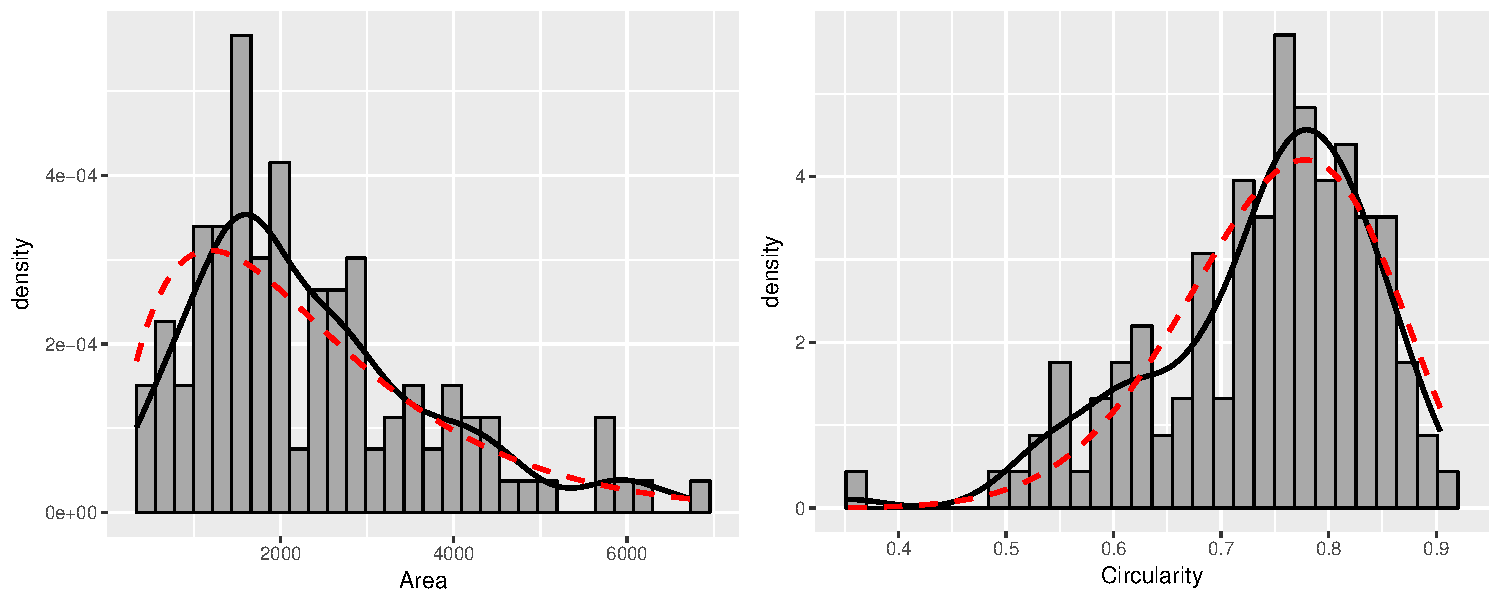
\includegraphics[width=\maxwidth]{figure/unnamed-chunk-1-1} 

\end{knitrout}
  \caption{Histogram of Area and Circularity}
  \small
  The red dash line at the left if is $Gamma(2, 1183)$; the one at the right is $Beta(15, 5)$ distribution.
  \label{fig_area_cir}
\end{figure}

\newpage
The following is a brief introduction about how to calculate 2nd Order Taylor's Approximation Estimator of ${\mu}_{P}$.

\noindent 
By Taylor's series expanded on ${\mu}_{A}$ and ${\mu}_{C}$ for 2nd order,
\begin{align*}
\begin{split}
E(P) &\doteq E(\sqrt{4 \pi}\left[ f({\mu}_{A},{\mu}_{C})+\frac{1}{1!}\big({f}_{x}({\mu}_{A},{\mu}_{C})(x-{\mu}_{A})+ {f}_{y}({\mu}_{A},{\mu}_{C})(y-{\mu}_{C}) \big) \right.\\
& \left. +\frac{1}{2!} \big( {f}_{xx}({\mu}_{A},{\mu}_{C}){(x-{\mu}_{A})}^2+ {f}_{yy}({\mu}_{A},{\mu}_{C}){(y-{\mu}_{C})}^2+2{f}_{xy}({\mu}_{A},{\mu}_{C})(x-{\mu}_{A})(y-{\mu}_{C}) \big) \right ])\\
&\doteq \sqrt{4 \pi}\left[ \sqrt{\frac{{\mu}_{A}}{{\mu}_{C}}}- \frac{1}{8} ({\mu}_{A})^\frac{-3}{2}({\mu}_{C})^\frac{-1}{2}{Var(A)}+\frac{3}{8}({\mu}_{A})^\frac{1}{2}({\mu}_{C})^\frac{-5}{2}{Var(C)}\right ]
\end{split}
\end{align*}
Then, plug in the parameters with their MLEs,
\begin{align*}
\widehat{E(P)} \doteq \sqrt{4 \pi}\left[ \sqrt{\frac{\bar{A}/2}{\bar{C}}} - \frac{1}{8} (\frac{\bar{A}}{2})^\frac{-3}{2}(\bar{C})^\frac{-1}{2}\frac{{s}_{A}^2}{2}+\frac{3}{8}(\frac{\bar{A}}{2})^\frac{1}{2}(\bar{C})^\frac{-5}{2}{s}_{C}^2\right].
\end{align*}

\end{document}
